\begin{figure}[t]
\centering

\begin{minipage}{0.48\linewidth}{
    \centering
    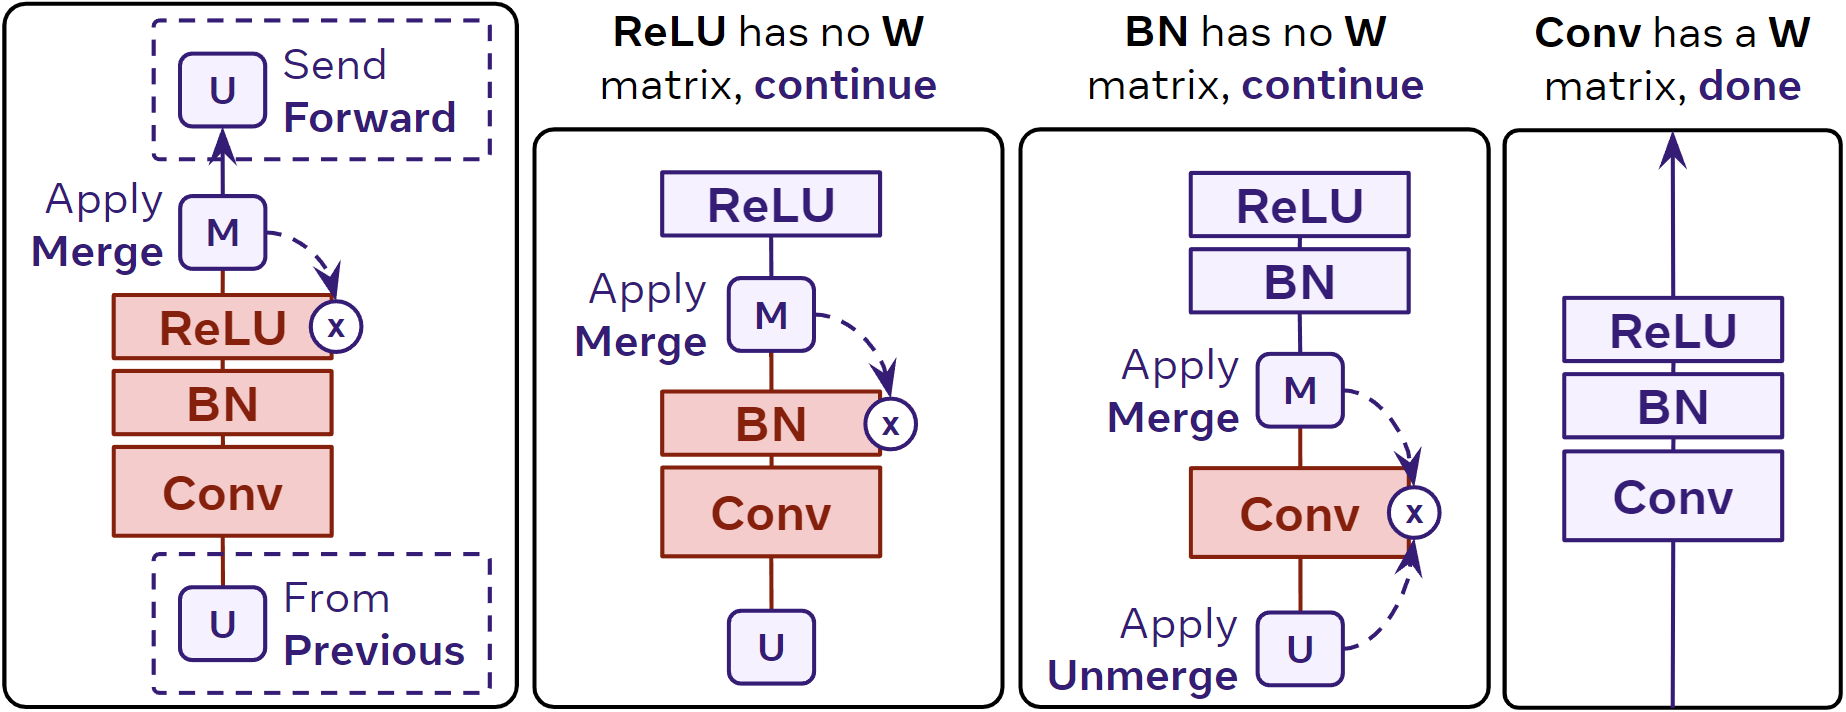
\includegraphics[width=\linewidth]{figures/imgs/zip_prop.png}
    \caption{{\bf Zip Propagation.} 
    % In practice, we compute \modelc{$M_i$} and \modelc{$U_i$} after activations (e.g., ReLU). 
    We propagate \modelc{$M_i$} backward until we hit a layer with weights, merging merging element-wise layers (e.g., BatchNorm) along the way.
    % We can't apply Eq.~\ref{eq:zip} to a layer without a weight matrix and have to propagate \modelc{$M_i$} backward until we hit such a layer. all element-wise layers (e.g., BatchNorm) are merged along the way.
    % Since we can't apply Eq.~\ref{eq:zip} to a layer without a weight matrix, we have to propagate \modelc{$M_i$} backward until we hit such a layer, merging element-wise layers (e.g., BatchNorm) along the way.
    }
    \label{fig:zip_prop}
}\end{minipage}
\hspace{1em}
\begin{minipage}{0.48\linewidth}{
    \centering
    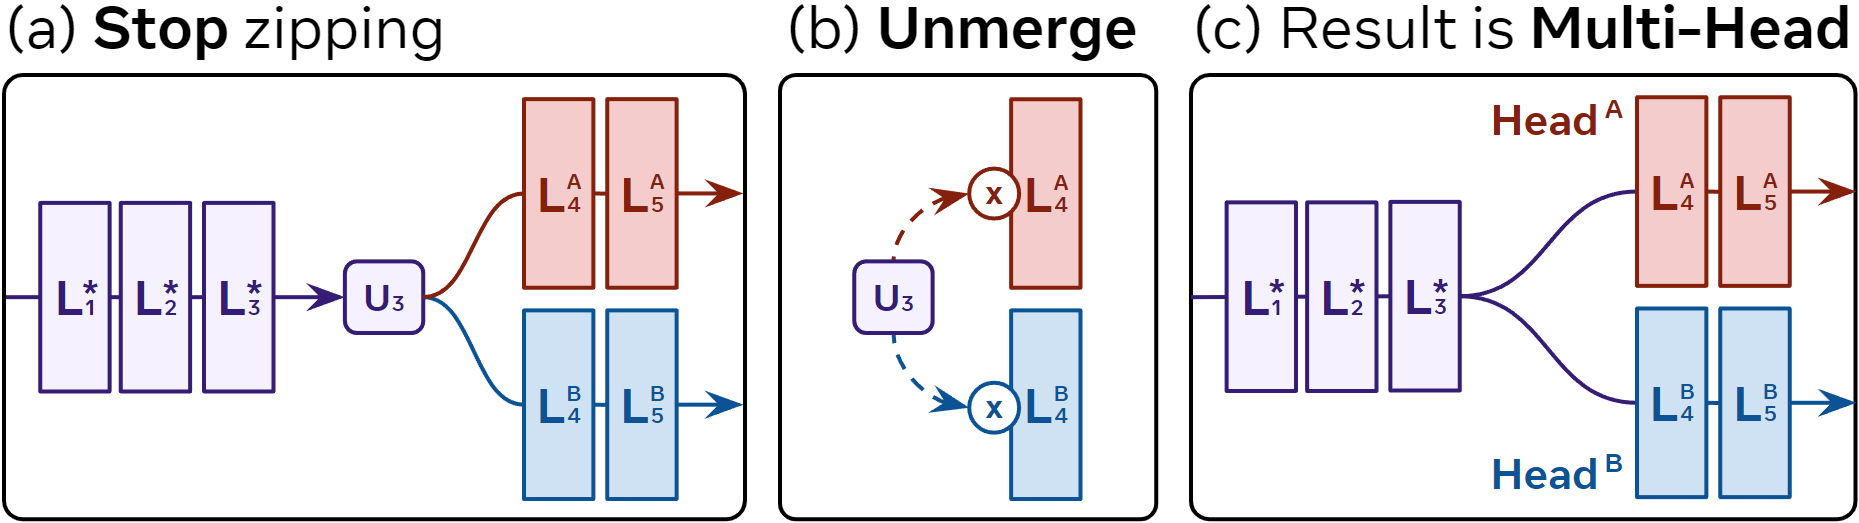
\includegraphics[width=\linewidth]{figures/imgs/partial_zip.png}
    \caption{
        {\bf Partial Zip.}
        (a) If we stop zipping early and (b) apply the latest \modelc{U} from the zip propagation to the inputs of the first unmerged layer in each model, (c) we get a multi-head model with a head for each task.
        % If we stop zipping early (a), we can create a multi-head model that can perform multiple tasks. All we need to do is apply the last unmerge from zip propogation (Fig.~\ref{fig:zip_prop}) to the inputs of the first unmerged layer in each model (b), and we get a model with multiple heads (c).
    }
    \label{fig:partial_zip}
}\end{minipage}
\vspace{-10pt}
\end{figure}
